\subsection{Kiến trúc hệ thống}
\subsubsection{Phân tích kiến trúc hệ thống phổ biến hiện nay}
Hiện nay, có nhiều kiến trúc phần mềm khác nhau, mỗi loại có ưu và nhược điểm riêng, phù hợp với các loại dự án và yêu cầu cụ thể. Dưới đây là một số kiến trúc phần mềm phổ biến và các điểm chính của chúng:
\begin{enumerate}
    \item Kiến trúc Monolithic
    \begin{itemize}
        \item \textbf{\textit{Định nghĩa:}} Kiến trúc monolithic là một mô hình truyền thống trong đó toàn bộ ứng dụng được xây dựng như một đơn vị duy nhất, tích hợp chặt chẽ.
        \item \textbf{\textit{Điểm chính:}} 
        \begin{itemize}
            \item Đơn giản để phát triển, triển khai và kiểm thử
            \item Hiệu suất tốt do không có overhead của network calls
            \item Khó mở rộng và bảo trì khi ứng dụng phức tạp
            \item Khó áp dụng công nghệ mới cho từng phần của ứng dụng
        \end{itemize}
        \item \textbf{\textit{Ví dụ:}} Một ứng dụng web PHP truyền thống, nơi tất cả chức năng (UI, business logic, data access) đều nằm trong cùng một codebase.
    \end{itemize}
    \item Kiến trúc Microservices
    \begin{itemize}
        \item \textbf{\textit{Định nghĩa:}} Kiến trúc microservices chia nhỏ ứng dụng thành các dịch vụ độc lập, mỗi dịch vụ chịu trách nhiệm cho một chức năng cụ thể và có thể được phát triển, triển khai độc lập.
        \item \textbf{\textit{Điểm chính:}} 
        \begin{itemize}
            \item Dễ dàng mở rộng và bảo trì từng service riêng biệt
            \item Cho phép sử dụng công nghệ phù hợp nhất cho mỗi service
            \item Tăng cường khả năng chịu lỗi của hệ thống
            \item Phức tạp hơn trong việc quản lý và điều phối các service
        \end{itemize}
        \item \textbf{\textit{Ví dụ:}} Netflix sử dụng kiến trúc microservices, với các service riêng biệt cho việc xử lý video, quản lý người dùng, đề xuất nội dung, v.v.
    \end{itemize}
    \item Kiến trúc Client-Server
    \begin{itemize}
        \item \textbf{\textit{Định nghĩa:}} Kiến trúc client-server chia ứng dụng thành hai phần chính: client (trình bày và tương tác người dùng) và server (xử lý logic nghiệp vụ và lưu trữ dữ liệu).
        \item \textbf{\textit{Điểm chính:}} 
        \begin{itemize}
            \item Phân tách rõ ràng giữa client và server
            \item Dễ dàng mở rộng server để đáp ứng nhu cầu người dùng
            \item Cải thiện bảo mật thông qua kiểm soát truy cập tại server
            \item Phụ thuộc vào kết nối mạng giữa client và server
        \end{itemize}
        \item \textbf{\textit{Ví dụ:}} Một ứng dụng web với frontend (React) và backend (Node.js) giao tiếp qua RESTful API.
    \end{itemize}
    \item Kiến trúc Event-Driven
    \begin{itemize}
        \item \textbf{\textit{Định nghĩa:}} Kiến trúc event-driven là một mô hình trong đó việc tạo ra, phát hiện, tiêu thụ và phản ứng với các sự kiện là cốt lõi của hệ thống.
        \item \textbf{\textit{Điểm chính:}} 
        \begin{itemize}
            \item Tách rời các thành phần hệ thống, giảm sự phụ thuộc trực tiếp
            \item Khả năng mở rộng và linh hoạt cao
            \item Dễ dàng thêm chức năng mới mà không ảnh hưởng đến các thành phần hiện có
            \item Có thể phức tạp trong việc theo dõi luồng xử lý và debug
        \end{itemize}
        \item \textbf{\textit{Ví dụ:}} Hệ thống thương mại điện tử, khi một đơn hàng được đặt, một sự kiện "OrderPlaced" được phát ra, kích hoạt các quy trình xử lý khác như cập nhật kho, gửi email xác nhận, v.v.
    \end{itemize}
    \item Kiến trúc Serverless
    \begin{itemize}
        \item \textbf{\textit{Định nghĩa:}} Kiến trúc serverless cho phép phát triển và chạy ứng dụng mà không cần quản lý trực tiếp máy chủ, tập trung vào việc viết code cho các chức năng (functions) cụ thể.
        \item \textbf{\textit{Điểm chính:}} 
        \begin{itemize}
            \item Giảm chi phí vận hành và bảo trì hạ tầng
            \item Tự động mở rộng theo nhu cầu sử dụng
            \item Chỉ trả tiền cho tài nguyên thực sự sử dụng
            \item Có thể gặp vấn đề về cold start và vendor lock-in
        \end{itemize}
        \item \textbf{\textit{Ví dụ:}} Một ứng dụng xử lý ảnh sử dụng AWS Lambda để thực hiện các tác vụ như resize, filter, và lưu trữ ảnh khi người dùng tải lên.
    \end{itemize}
\end{enumerate}

\subsubsection{Lựa chọn kiến trúc hệ thống}
Dựa trên yêu cầu của hệ thống, nhóm quyết định sử dụng kiến trúc Client-Server. Cụ thể như sau:
\begin{enumerate}
    \item Client Tier:
    \begin{itemize}
        \item \textbf{Frontend:} Ứng dụng Vue.js cung cấp giao diện người dùng cho sinh viên, giảng viên và admin.
        \item \textbf{Chức năng:} Hiển thị nội dung học tập, quản lý khóa học, bài tập, lộ trình học tập và tương tác với người dùng.
        \item \textbf{Tương tác:} Giao tiếp với server thông qua RESTful API.
    \end{itemize}
    \item Server Tier:
    \begin{enumerate}
        \item \textbf{API Layer:}
        \begin{itemize}
            \item \textbf{Framework:} FastAPI xử lý các yêu cầu từ client.
            \item \textbf{Chức năng:}
            \begin{itemize}
                \item \textit{User Management:} Quản lý thông tin người dùng, xác thực và phân quyền.
                \item \textit{Course Management:} CRUD cho khóa học, module, bài học và nội dung học tập.
                \item \textit{Recommendation System:} Đề xuất tài nguyên học tập dựa trên dữ liệu người dùng.
                \item \textit{AI Tutor:} Tích hợp LangChain để hỗ trợ giải đáp thắc mắc và giải thích mã nguồn.
                \item \textit{Exercise Generation:} Tạo bài tập và test cases tự động bằng LangChain.
                \item \textit{Progress Tracking:} Theo dõi tiến độ học tập và tạo báo cáo.
            \end{itemize}
        \end{itemize}
        \item \textbf{Persistence Layer:}
        \begin{itemize}
            \item \textbf{PostgreSQL:} Lưu trữ dữ liệu có cấu trúc như thông tin người dùng, khóa học, bài học và tiến độ học tập.
            \item \textbf{AWS S3:} Lưu trữ tài liệu học tập, video bài giảng và các tài nguyên khác.
        \end{itemize}
        \item \textbf{Caching Layer:}
        \begin{itemize}
            \item \textbf{Redis:} Lưu trữ tạm thời dữ liệu thường xuyên truy cập để cải thiện hiệu suất và giảm tải cho cơ sở dữ liệu.
        \end{itemize}
    \end{enumerate}
\end{enumerate}

\textbf{\textit{Phân tích nguyên nhân:}}
\begin{itemize}
    \item \textbf{Phân tách rõ ràng:} Kiến trúc Client-Server tách biệt giữa giao diện người dùng (client) và logic nghiệp vụ/dữ liệu (server), giúp dễ dàng phát triển và bảo trì.
    \item \textbf{Dễ mở rộng:} Server có thể được mở rộng bằng cách tăng tài nguyên hoặc thêm các instance FastAPI khi số lượng người dùng tăng.
    \item \textbf{Bảo mật:} Server kiểm soát truy cập và xác thực, đảm bảo an toàn dữ liệu.
    \item \textbf{Hiệu quả:} Sử dụng Redis để tối ưu hiệu suất truy vấn và AWS S3 để quản lý tài nguyên lớn như video, tài liệu.
\end{itemize}

\textbf{\textit{Không dùng:}}
\begin{itemize}
    \item \textit{Monolithic:} Khó mở rộng, bảo trì và tích hợp công nghệ mới khi hệ thống phát triển.
    \item \textit{Microservices:} Phức tạp trong quản lý nhiều dịch vụ, không cần thiết cho quy mô hiện tại của hệ thống.
    \item \textit{Event-Driven:} Phức tạp trong việc đồng bộ và theo dõi trạng thái, không phù hợp với yêu cầu tương tác trực tiếp.
    \item \textit{Serverless:} Phụ thuộc nhà cung cấp, chi phí cao khi tải tăng và hạn chế tùy chỉnh hiệu suất.
\end{itemize}

\textbf{\textit{Luồng hoạt động:}}
\begin{itemize}
    \item Người dùng tương tác với giao diện Vue.js (Client Tier).
    \item Client gửi các request đến server thông qua RESTful API.
    \item FastAPI (Server Tier) xử lý logic nghiệp vụ, truy vấn PostgreSQL hoặc AWS S3 để lấy/lưu dữ liệu.
    \item Redis được sử dụng để cache dữ liệu, giảm thời gian phản hồi.
    \item Kết quả được trả về client để hiển thị cho người dùng.
\end{itemize}

\textbf{\textit{Tóm lại,}} kiến trúc Client-Server được chọn vì sự đơn giản, khả năng mở rộng và tính bảo mật cao, phù hợp với yêu cầu của hệ thống học tập trực tuyến thông minh. Việc sử dụng Vue.js, FastAPI, PostgreSQL, AWS S3 và Redis đảm bảo hiệu suất, linh hoạt và dễ dàng bảo trì trong tương lai.
\begin{figure}[H]
    \centering
    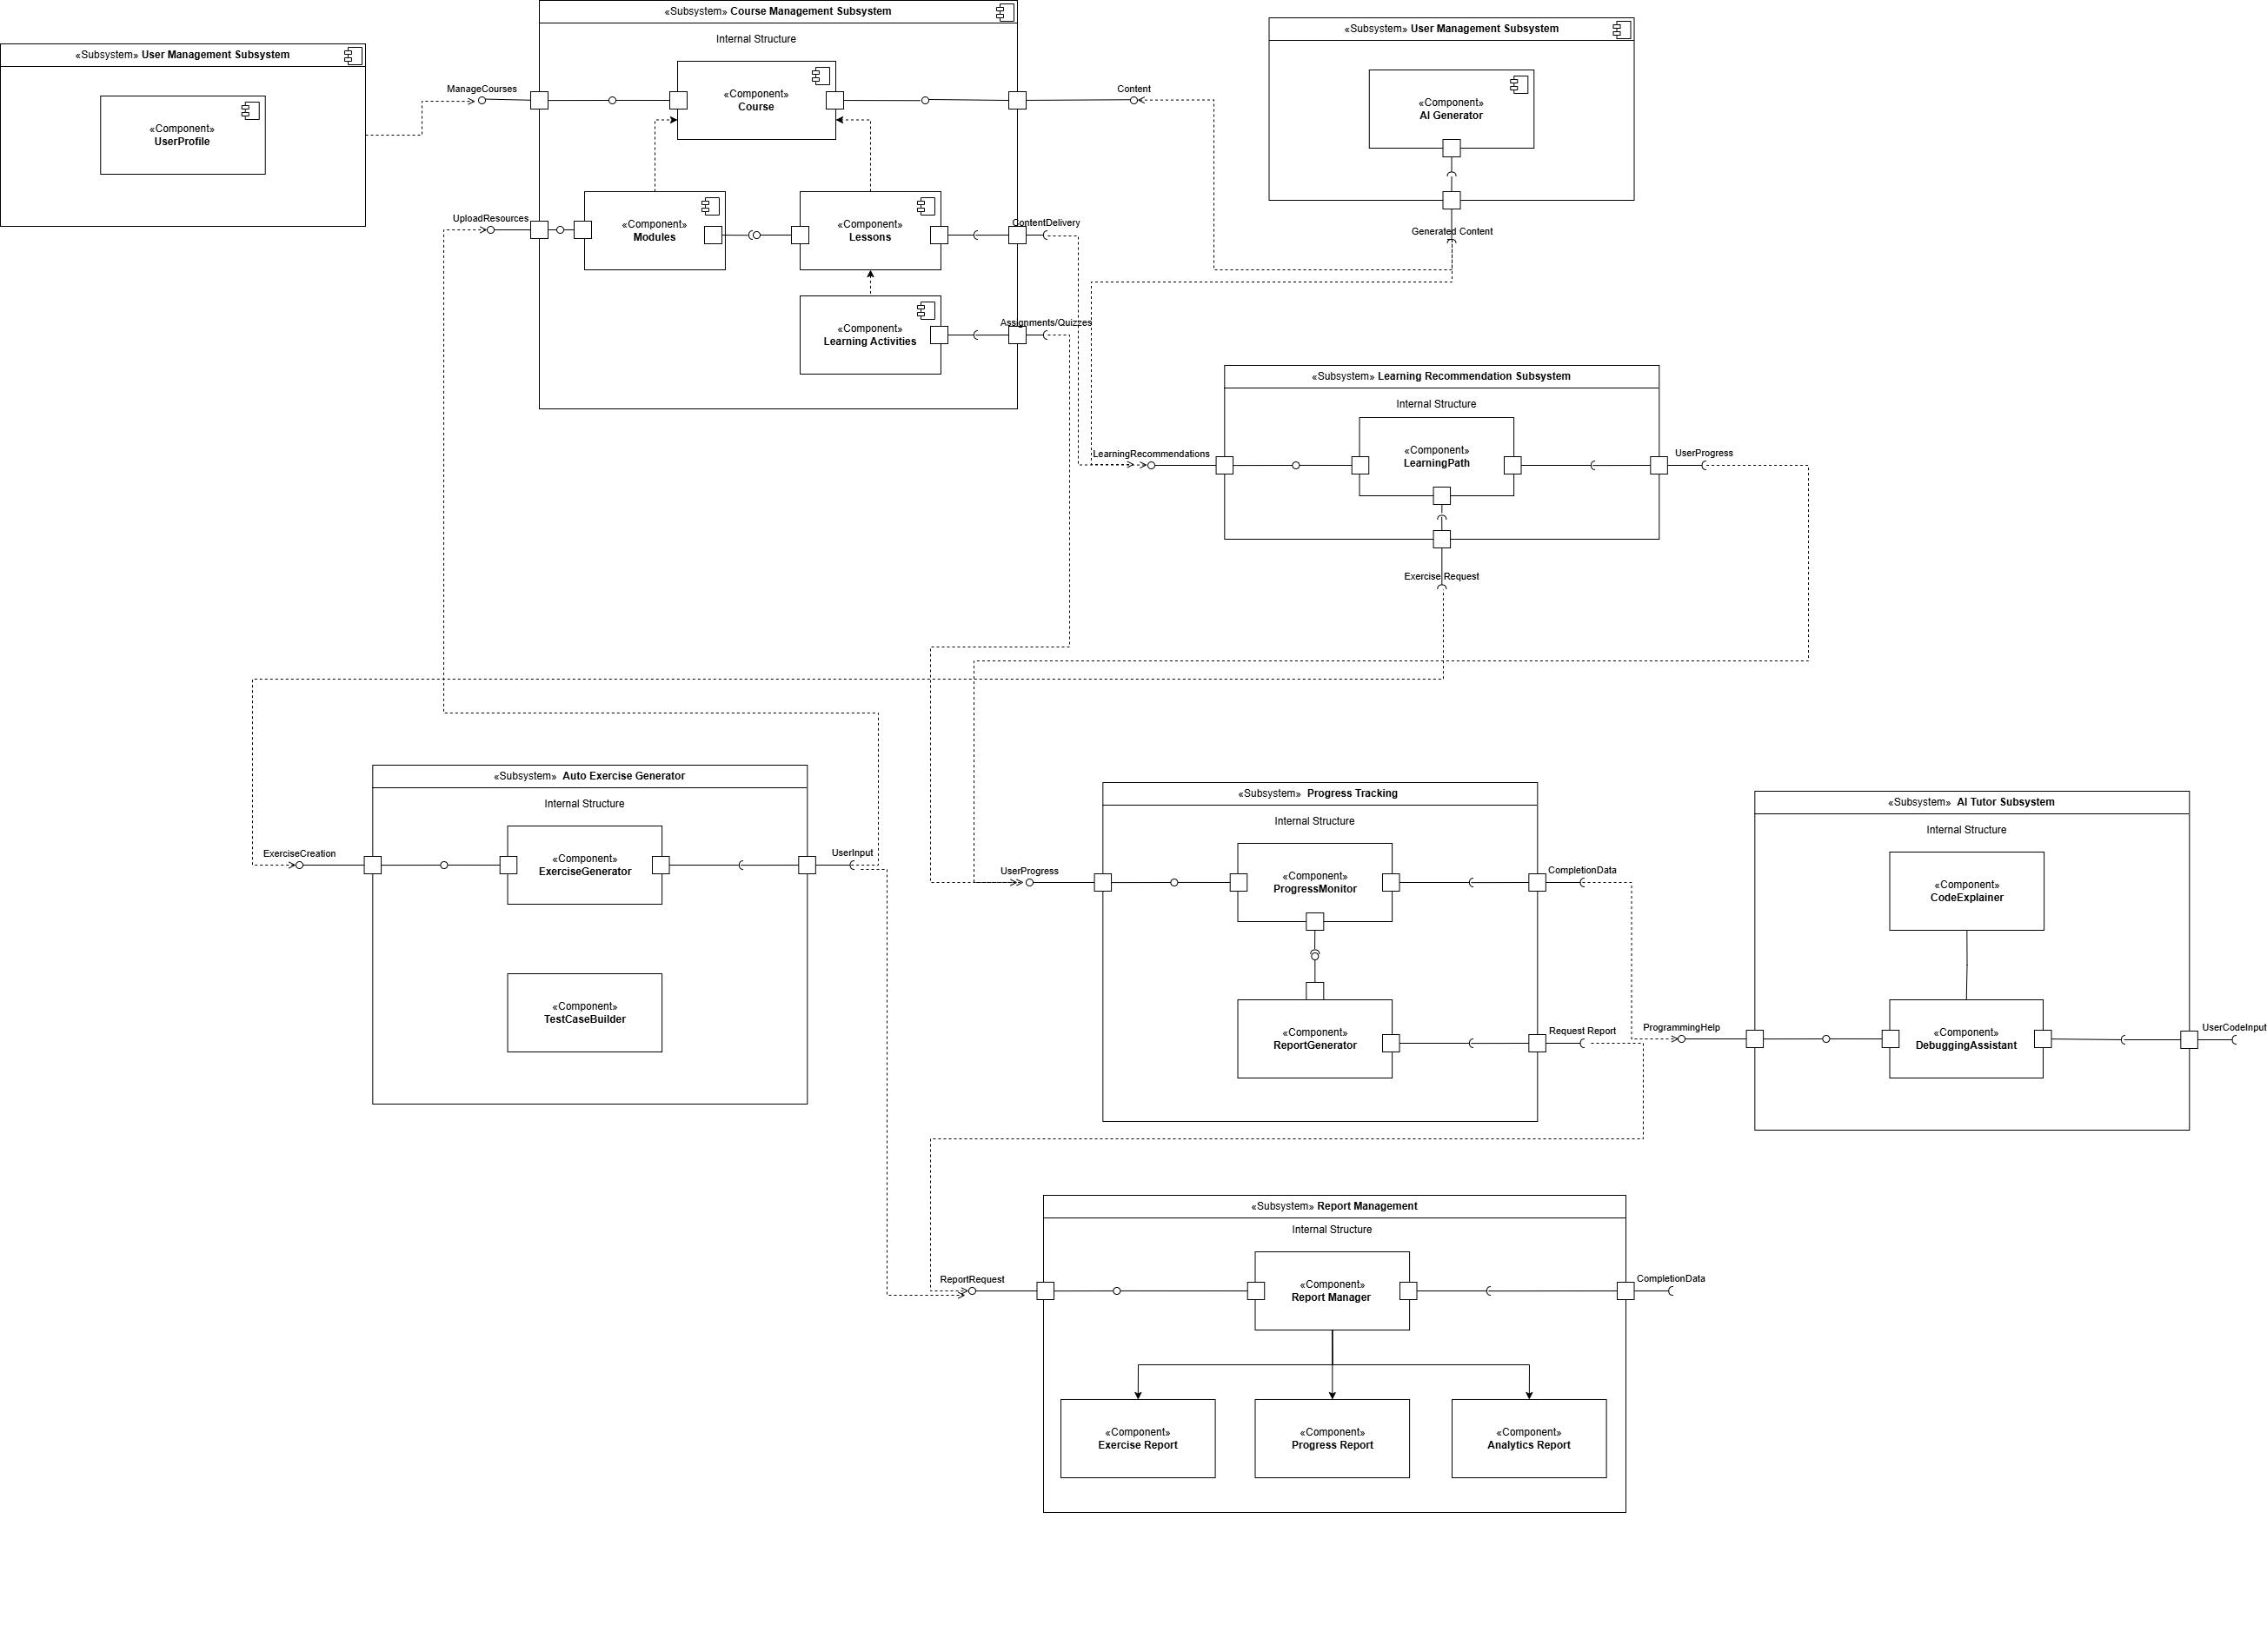
\includegraphics[width=\linewidth]{Images/component_diagram/component-All.drawio.png}
    \caption{Component-based Diagram cho toàn bộ hệ thống}
    \label{fig:enter-label}
\end{figure}
\begin{figure}[H]
    \centering
    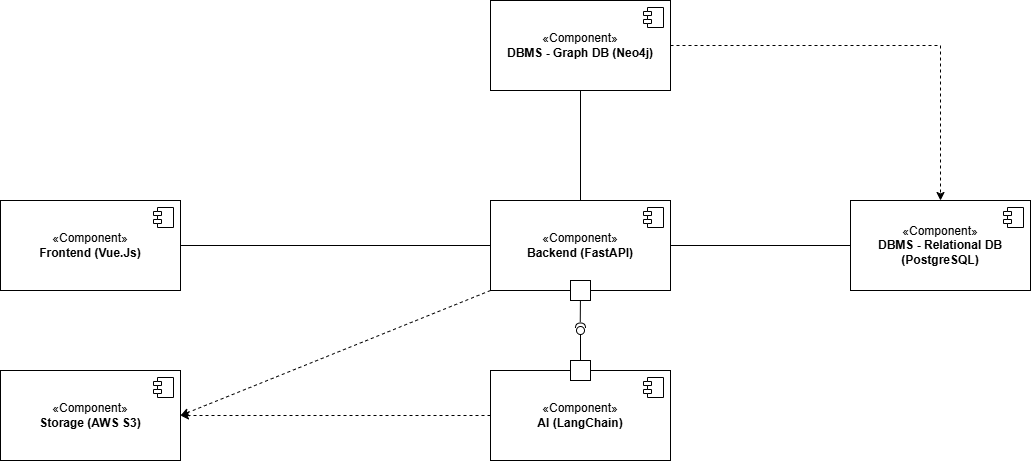
\includegraphics[width=\linewidth]{Images/component_diagram/component-Selected technologies.drawio.png}
    \caption{Component-based Diagram cho những công nghệ được chọn}
    \label{fig:enter-label}
\end{figure}